\chapter{Опис додатку з використанням кросс-платформених рішень}
\label{ch2}


\section{Структура проекту в React Native}
\label{section.2.1}

\begin{lstlisting}[style=light, language=Python,label={lst:rn_app_structure},caption=React Native App Layout]
├── App.js (1)
├── Readme.md
├── __tests__ (2)
│ └── App.js
├── android (3)
│ ├── app
│ ├── build
│ ├── build.gradle
│ ├── gradle
│ ├── gradle.properties
│ ├── gradlew
│ ├── gradlew.bat
│ ├── local.properties
│ └── settings.gradle
├── app.json (5)
├── babel.config.js (6)
├── index.js (7)
├── ios (4)
│ ├── BreedRN
│ ├── BreedRN.xcodeproj
│ ├── BreedRN.xcworkspace
│ ├── Podfile
│ ├── Podfile.lock
│ └── Pods
├── metro.config.js (8)
├── node_modules (11)
├── package-lock.json (10)
└── package.json (9)
\end{lstlisting}

\begin{enumerate}
    \item \textbf{App.js} сирцевий код нашого додатку
    \item \textbf{\_\_tests\_\_} сирцевий код тестів
    \item \textbf{android} сирцевий код платформеного коду Android
    \item \textbf{ios} сирцевий код платформеного коду iOS
    \item \textbf{app.json} конфігурує багато речей, від назви вашого додатка до піктограми до заставки, і навіть схеми глибоких зв’язків та ключів API для використання для деяких служб
    \item \textbf{babel.config.js} конфігурує Babel - це набір інструментів, який в основному використовується для перетворення коду ECMAScript 2015+ у зворотну сумісну версію JavaScript у поточних та старих браузерах або середовищах.
    \item \textbf{index.js} точка входу для React Native з цього файлу Javascript Engine вивантажує в пам'ять логіку додатку
    \item \textbf{metro.config.js} конфігурує Metro пакувальник JavaScript для платформ Android та iOS
    \item \textbf{package.json} конфігурує дерево залежностей або бібліотек, що використовує проект
    \item \textbf{package-lock.json} файл що описує повністю дерево залежностей, таким чином створює відтворюване середовище
    \item \textbf{node\_modules} репозиторій артефактів або сирцевого коду всіх Javascript пакетів, що використовує проект
\end{enumerate}


\section{Структура проекту в Flutter}
\label{section.2.2}

\begin{lstlisting}[style=light, language=Python,label={lst:flutter_project_layout},caption=Flutter Project Layout]
├── README.md
├── android (1)
│ ├── app
│ ├── build.gradle
│ ├── gradle
│ ├── gradle.properties
│ ├── gradlew
│ ├── gradlew.bat
│ ├── local.properties
│ └── settings.gradle
├── build (2)
├── ios (3)
│ ├── Flutter
│ ├── Podfile
│ ├── Runner
│ ├── Runner.xcodeproj
│ └── Runner.xcworkspace
├── lib (4)
│ ├── breed_list.dart
│ ├── data
│ ├── domain
│ ├── home.dart
│ ├── main.dart
│ └── presentation
├── pubspec.lock (5)
├── pubspec.yaml (6)
├── test (7)
│ ├── breed_database_test.dart
│ ├── breed_list_view_model_test.dart
│ ├── breed_list_view_model_test.mocks.dart
│ └── network_test.dart
└── web (8)
    ├── favicon.png
    ├── icons
    ├── index.html
    └── manifest.json
\end{lstlisting}

\begin{enumerate}
    \item \textbf{android} сирцевий код платформеного коду Android.
    \item \textbf{build} папка з тимчасовими файлами згенерованими Flutter CLI під час побудування проекту.
    \item \textbf{ios} сирцевий код платформеного коду iOS.
    \item \textbf{lib} сирцевий код Flutter, котрий фактично є серцем репозиторія та описую логіку проекту.
    \item \textbf{pubspec.lock} файл що описує повністю дерево залежностей, таким чином створює відтворюване середовище.
    \item \textbf{pubspec.yaml} конфігурує дерево залежностей або бібліотек, що використовує проект.
    \item \textbf{test} сирцевий код тестів для платформи Flutter.
    \item \textbf{web} сирцевий код платформеного коду веб сторінки.
\end{enumerate}


\section{Структура проекту Kotlin Multi-Platform}
\label{section.2.3}

\begin{lstlisting}[style=light, language=Python,label={lst:kmm_project_layout},caption=KMM Project Layout]
├── app (1)
│ ├── build.gradle.kts
│ └── src
├── build.gradle.kts
├── buildSrc (2)
│ ├── build.gradle.kts
│ └── src
├── gradle
├── gradle.properties
├── gradlew
├── gradlew.bat
├── ios (3)
│ ├── Podfile
│ ├── Podfile.lock
│ ├── Pods
│ ├── bai_dialog_ios
│ ├── bai_dialog_ios.xcodeproj
│ ├── bai_dialog_ios.xcworkspace
│ ├── bai_dialog_iosTests
│ └── bai_dialog_iosUITests
├── local.properties
├── settings.gradle.kts
└── shared (4)
    ├── build.gradle.kts
    ├── consumer-rules.pro
    ├── proguard-rules.pro
    ├── shared.podspec
    └── src
        ├── androidMain (5)
        ├── androidTest (6)
        ├── commonMain (7)
        ├── commonTest (8)
        ├── iosMain (9)
        ├── iosTest (10)
        └── main (11)
\end{lstlisting}

\begin{enumerate}
    \item \textbf{app} сирцевий код UI імплементації для Android.
    \item \textbf{buildSrc} сирцевий код, що розширює систему розгортання Gradle.
    \item \textbf{ios} сирцевий код UI імплементації для iOS.
    \item \textbf{shared} папка в котрій зберігається загальний код.
    \item \textbf{androidMain} імплементація коду специфічного для Android платформи.
    \item \textbf{androidTest} імплементація тестів специфічних для Android платформи.
    \item \textbf{commonMain} сирцевий код спільної незалежної від платформи логіки.
    \item \textbf{commonTest} імплементація тестів для спільної незалежної від платформи логіки.
    \item \textbf{iosMain} імплементація коду специфічного для iOS платформи.
    \item \textbf{iosTest} імплементація тестів специфічних для iOS платформи.
    \item \textbf{main} репозиторій в якому зберігається код Android модуля, а саме статичні ресурси та AndroidManifest.
\end{enumerate}


\section{Архітектура додатку React Native}
\label{section.2.4}
В реалізації додатку React Native ми використали систему звротніх викликів або так званих "хуків".
Наприклад, \textbf{useState} - це Хук, що дозволяє додавати стан React до функціональних компонентів.

"useState" оголошує "змінну стану" та повертає пару значень: поточний стан та функцію, яка його оновлює.
Наша змінна називається, data ми можемо називати її як завгодно, наприклад banana \ref{lst:rn_state_hooks}.

Використовуючи useEffect хук, ми повідомляємо React, що наш компонент повинен виконати додаткову фунцію після рендерингу.
React запам'ятає передану нами функцію (яку ми будемо називати "ефектом") і викличе її пізніше після оновлення UI нашого додатку.

Ефект котрий ми створили буде виконаний при ініціалізації додатку. І як результат виконання ми отримаємо дані з локальної бази які ми і відобразимо (див. на \ref{fig:rn_realm})).

\begin{figure}
    \begin{center}
        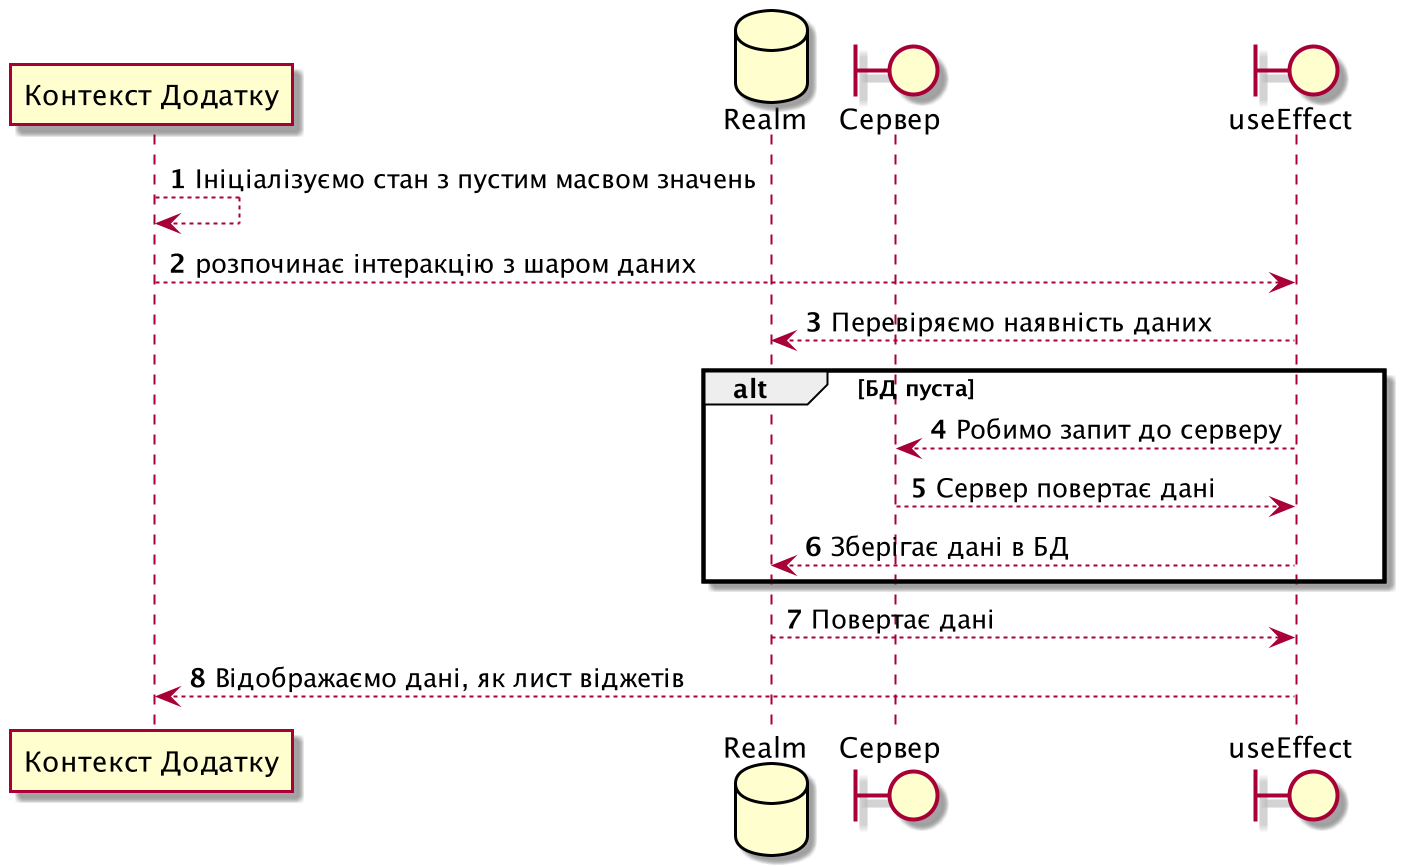
\includegraphics[scale=0.3]{app_widget.png}
        \caption{Схема послідовності віджету App та інтеракція з шаром даних}
        \label{fig:rn_realm}
    \end{center}
\end{figure}


\section{Комунікація з мережею в Flutter додатку з http.dart та async/await}
\label{section.2.5}
В нашому додатку запит до інтернету описан в наступному описі сирцевого коду \ref{lst:flutter_networking}.

Найголовнішим принципом, котрим ми опируємо в прикладі запиту до інтернету, це використання "обіцянок" на базі dart:async Future<T>.
Асинхронні операції дозволяють нашій програмі завершити роботу, чекаючи закінчення іншої операції.
Результат використання Future API або закінчиться в завершенному стані або незавершенному.

Коли ми вперше виконуємо асинхрону функцію, то отримаємо посилання на незавершену дію, з якої ми очікуємо результат або помилку.
Щоб уникнути розповсюдження помилки до верхнів шарів ми маємо використати try/catch синтаксис.

Як видно з нашого прикладу використання пакету http.dart в по'єднанні з dart:async дає зручне
та швидке розв'язання проблеми створення та прослухання результатів з інтернету.


\section{Комунікація з SQLite БД в Flutter додатку з SQFlite}
\label{section.2.6}
Для комунікації з БД в додатку була використана бібліотека SQFlite.
Рішення, що використовує цю бібліотеку можна знайти за наступним посиланнєм \ref{lst:flutter_sqflite}.

Для того щоб, уникнути витік залежності рішення SQFlite було огорнуто в додатковий тип \textbf{BreedDatabase}.
\textbf{BreedDatabase} дає можливість виконання стандартних процедур підключення до БД з розширенням .sqlite
на стандартному шляху до файлу абстрагованого за допомогою \textbf{getDatabasesPath()} API.

Оскільки наша огортка, це вікно в SQL світ, то наш додаток здатен виконувати всі доступні із стандартного набору
SQL операції.


\section{Управління станом в Flutter додатку з Providers API}
\label{section.2.7}
Flutter пропонує кілька способів для управління станом. Серед них BLoC, Provider, Statefull Widgets, InheritedWidgets.
В даній роботі ми розглянемо Provider API, котрий взяв за основу систему InheritedWidgets(віджет, що наслідує).
Для того щоби зрозуміти контроль стану з Provider API ми повинні розлянути:

\begin{itemize}
    \item ChangeNotifier - це простий клас, включений до Flutter SDK, який забезпечує повідомлення про зміни своїх слухачів. Іншими словами, якщо щось є ChangeNotifier, ви можете підписатися на його зміни.
    \item ChangeNotifierProvider - це віджет, який надає екземпляр ChangeNotifier своїм нащадкам. Це походить від пакету провайдера.
    \item Consumer - це віджет, що дозволяє нам огорнути будь-який інший віджит далі в ієрархії та зчитати стан з класу, що наслідує ChangeNotifier.
\end{itemize}

В нашому додатку ми використали StateNotifier, котрий обновлює всіх підписників стану.
Так наприклад зміна значення з стану "завантажується" на стан "завантажений" приводить до перебудови віджету \ref{lst:flutter_sqflite}.


\section{Юніт тестування в Flutter додатку}
\label{section.2.8}
Як було вже зазначено, найкращий спосіб контролю якості в проекті це написання та сопроводження коду написанням юнит тестів.
Цей підхід до розробки програмного забезпечення не оминув і розробку під Flutter.

В даній секції ми наведемо приклад тесту написаного для коду бізнес логіки \ref{lst:flutter_unit_test}.
Ми застосуємо пакети test та mockito.
Пакет тест надає доступ до функцій, які дозволяють нам групувати тести.
Пакет mockito надає функціонал, що дозволяє конфігурувати поведінку об'єктів типу mock(заглушка).

Ми маємо дві "рухомі" залежності: шар комунікації з мережею та БД.
Рухомі частини - це те що ми, як користувачі бібліотек http.dart та SQFlite не контролюємо.
Отже, щоб спростити конфігурацію юніт тестування ми замінили реальні об'єкти на об'єкти заглушки.


\section{UI та Kotlin Multiplatform}
\label{section.2.8}
Специфіка розробки з використанням Kotlin Multiplatform передбачує, що розробка рівня UI буде досягнута
інструментами нативними для платформи.

Для розробки UI під Android використовується декларативний XML, що відтворюється під час виконання в середовищі компоненту
контейнера так званої Activity(активність).
\begin{lstlisting}[style=light, language=Python,label={lst:android_xml},caption=Android UI with XML]
// 1
class MainActivity : AppCompatActivity() {
    override fun onCreate(savedInstanceState: Bundle?) {
        super.onCreate(savedInstanceState)
        // 2
        setContentView(R.layout.activity_main)
    }
}

// 3
<?xml version="1.0" encoding="utf-8"?>
<androidx.constraintlayout.widget.ConstraintLayout
    xmlns:android="http://schemas.android.com/apk/res/android"
    xmlns:app="http://schemas.android.com/apk/res-auto"
    xmlns:tools="http://schemas.android.com/tools"
    android:layout_width="match_parent"
    android:layout_height="match_parent"
    tools:context=".MainActivity"/>
\end{lstlisting}

\begin{enumerate}
    \item Декларуємо клас, що наслідує Activity.
    \item Конфігуруємо Activity посилаючись на XML, що визначає елементи UI.
    \item Безпосередньо сам XML, що декларує опис розмітки.
\end{enumerate}

Нещодавно з'явився тренд розробки UI з уживанням
Kotlin DSL(Domain Specific Language - Специфічна Мова Домену) так званий Jetpack Compose \cite{jetpack_compose}.

\begin{lstlisting}[style=light, language=Python,label={lst:android_jetpack_compose},caption=Android Jetpack Compose]
class MainActivity : AppCompatActivity() {
    override fun onCreate(savedInstanceState: Bundle?) {
        super.onCreate(savedInstanceState)

        val appContainer = (application as JetnewsApplication).container
        // 1
        setContent {
            // 2
            JetnewsApp(appContainer, navigationViewModel)
        }
    }
}
\end{lstlisting}

\begin{enumerate}
    \item Викликаємо функцію setContent, що приймає як аргумент функцію, що створює віджет.
    \item Створюємо віджет, який описує додаток.
\end{enumerate}

Як видно з прикладу \ref{android_jetpack_compose} Android екосистема взяла той самий керунок, що Flutter та React Native.
Такий самий тренд можна спостерігати і в розробці під iOS, де декларативний синтаксис описується з Swift UI \cite{swift_ui}.

\begin{lstlisting}[style=light, language=Python,label={lst:ios_swift_ui},caption=Swift UI]
import SwiftUI

// 1
@main
struct LandmarksApp: App {
    // 2
    var body: some Scene {
       // 3
        WindowGroup {
            ContentView()
        }
    }
}
\end{lstlisting}

\begin{enumerate}
    \item Декларуємо структуру, що є вхідною точкою для запуску додатку.
    \item Декларуємо сцену, що визначає екран користувача.
    \item В декларативний спосіб описуємо UI.
\end{enumerate}

Як видно з прикладів \ref{android_jetpack_compose} та \ref{ios_swift_ui} Android та iOS теж вибрали стежку декларативної розробки UI.
В свою чергу стає зрозуміло, що Kotlin Multiplatform не розв'язує проблему спільної бази коду для коду UI.
Це дуже важливий момент, оскільки весь UI треба дуплікувати під кожну платформу.
Якщо Kotlin Multiplatform не розв'язує проблему, то для чого його використовувати?
Задачу яку собі поставив Kotlin Multiplatform, це опис спільної логіки, тобто звернення до бази даних, файлової системи, інернету, тощо.


\section{Система побудування Gradle}
\label{section.2.9}

Gradle - це система побудування проектів розроблена для рішення проблем побудування проектів зокрема для JVM платформ.
Gradle - це інструмент автоматизації збірки з відкритим кодом, орієнтований на гнучкість та продуктивність. \cite{gradle_user_manual}
Сценарії збірки Gradle пишуться із використанням DSL Groovy або Kotlin. \cite{gradle_user_manual}

Оскільки Kotlin спочатку був розроблен для JVM систем, то був на раніх етапах інтегрован в екосистему.
З розвитком Kotlin Multiplatform дана система була наслідувана і надалі використовується для побудування крос-платформеного проекту.

Якщо ви знайомі з проектами Android, то знаєте, що залежності та конфігурація побудування проекту можна знайти у build.gradle.

Оскільки shared модуль є бібліотекою для Android, він також містить власний build.gradle скрипт, де описані залежності.
Скрипт "shared/build.gradle.kts", описує конфігурації сирцевих кодів з використанням sourceSets, що відповідає каталогам у спільному проекті.

Кожна частина бібліотеки, оголошує власні залежності в визначених наборах джерел.
Наприклад, бібліотека параметрів мультиплатформних налаштувань оголошується лише у commonMain та commonTest,
оскільки бібліотека використовує метадані gradle для виведення залежних від конкретних платформ залежностей.
Інші бібліотеки, які залежать від реалізації платформи, наприклад SqlDelight, вимагають конфігурації яка задовольнить
умовам середи виконання.

Наприклад для sourceSet commonMain визначена залежність з пакету sqlDelight.runtime, а в androidMain sqlDelight.driverAndroid.


\section{Запити до мережі з Ktor}
\label{section.2.10}
На даний момент серед кроссплатформених бібліотек, що дозволяє нам моделювання інтернет викликів, найпоширенішою - є розв'язання Ktor \cite{ktor_home_page}.
В додатку коду, що йде нижче \ref{kmm_ktor} ми розглянемо приклад реалізації клієнта, що надалі створює з'єднання з API сервісом, що повертає нам список порід собак.

\begin{lstlisting}[style=light, language=Python,label={lst:kmm_ktor},caption=Ktor]
import io.ktor.client.HttpClient
import io.ktor.features.json.*
import io.ktor.request.*
import io.ktor.http.takeFrom

// 1
interface KtorApi {
    // 2
    suspend fun getJsonFromApi(): BreedResult
}

class DogApiImpl : KtorApi {
    // 3
    private val client = HttpClient {
        install(JsonFeature) { serializer = KotlinxSerializer() }
    }

    // 4
    init { ensureNeverFrozen() }

    // 5
    override suspend fun getJsonFromApi(): BreedResult =
        client.get<BreedResult> { url {
            takeFrom("https://dog.ceo/")
            encodedPath = "api/breeds/list/all"
        }
    }
}
\end{lstlisting}

\begin{enumerate}
    \begin{item}
        Визначаємо інтерфейс, що повертає нам результат виконання виклику до API.
    \end{item}

    \begin{item}
        Важливим момент є те, що функція визначена ключовим словом suspend.
        suspen маркерує нашу функцію, як ту, що буде виконувати "блокуючу" операцію.
        Виконання викликів до інтернету операція дорога і можевиконуватися секундами.
    \end{item}

    \begin{item}
        Створюємо об'єкт Ktor клієнта та конфігуруємо Json Serializer/Deserializer.
    \end{item}

    \begin{item}
        \textbf{ensureNeverFrozen} гарантує, що freezing(заморожування) закінчиться помилкою FreezingException.
        Дозволяє уникнути небажаного ефекту freezing, що є основою безпечного контролю посилань між паралельними потоками
        під час виконання програмою асинхроних викликів.
    \end{item}

    \begin{item}
        Реалізуємо функцію інтерфейсу декларуючи посилання, що нам поверне результат.
    \end{item}

\end{enumerate}

Як ми бачимо реалізація виклику за допомогою Ktor та Kotlin, хоча виглядає громоздко, але не є складною.
Більшість логіки, що створює сокет і опрацьовую потік байтів енкапсульвона за публічним інтерфейсом.
Від клієнта потребується декларування викликів та дизайн DTO(Data Transfer Object - Транспортний Об'єкт Даних),
в нащому випадку це клас, що описує структуру Json відповіді BreedResult.


\section{Запити до SQLite бази даних з SQLDelight}
\label{section.2.11}
Для роботи з БД в нашому KMM(Kotlin) проекті було використана SQLDelight рішення \cite{sqldelight_home}.
SQLDelight використовує ідею генерації коду клієнту на основі SQL визначень описаних в окремому файлі.

\begin{lstlisting}[style=light, language=Python,label={lst:table_sq},caption=Table.sq]
// 1
CREATE TABLE Breed (
    id INTEGER NOT NULL PRIMARY KEY AUTOINCREMENT,
    name TEXT NOT NULL,
    favorite INTEGER NOT NULL DEFAULT 0
);

// 2
selectAll:
// 3
SELECT * FROM Breed;
\end{lstlisting}

\begin{enumerate}
    \item SQL що описує структуру таблиці.
    \item Інструкція, що використовує SQLDelight для генерації Kotlin функції.
    \item SQL запит що буде використаний для виборки значень з таблиці.
\end{enumerate}

Як видно з прикладу \ref{table_sq_gen} визначений вище SQL запит був використаний в згенерованому коді.
Результатом виконання SQL запиту є посилання на об'єкт типу курсор, що дозволяє в динамічний спосіб зчитати
результат та адуптувати результат до конкретного типу.
Таким чином, ми уникаємо написання низькорівневого коду, в якому дуже просто припуститися помилки.

\begin{lstlisting}[style=light, language=Python,label={lst:table_sq_gen},caption=Generate code]
fun <T : Any> selectAll(mapper: (
  id: Long,
  name: String,
  favorite: Long
) -> T): Query<T> = Query(552535035, selectAll, driver, "Table.sq", "selectAll",
    "SELECT * FROM Breed") { cursor ->
  mapper(
    cursor.getLong(0)!!,
    cursor.getString(1)!!,
    cursor.getLong(2)!!
  )
}
\end{lstlisting}


\section{Юніт тестування в KMM}
\label{section.2.12}

Як і в випадку інших платформ розробки тестування коду є критичною для розвитку продукту.
KMM і тут не відстає і пропонує розв'язання для тестування.
Оскільк Kotlin підтримує JVM(Java Virtual Machine) середовище ми можемо запускати тести на стороні Linux, Windows та MacOS платформ.

Тести, що супроводжують загальну логіку тримають в відокремленому репозиторії commonTest.
Для конфігурації специфічного для платформи коду виділяють iosTest для iOS та androidTest для Android платформ.

\begin{lstlisting}[style=light, language=Python,label={lst:kotin_test_common},caption=Common Unit Test]
// 1
internal expect fun testDbConnection(): SqlDriver
// 2
internal expect fun <T> runTest(block: suspend () -> T)

abstract class SqlDelightTest {
    private lateinit var dbHelper: DatabaseHelper

    @BeforeTest
    fun setup() = runTest {
        // 3
        dbHelper = DatabaseHelper(testDbConnection())
    }
}
\end{lstlisting}

\begin{enumerate}
    \item Ф-ція \textbf{testDbConnection} абстрагує реалізацію драйверу.
    \item Ф-ція \textbf{runTest} абстрагує реалізацію логіку запуску тесту. Модель багатопотоковість унікальна для кожної з платформ.
    \item Безпосередньо створюємо об'єкт, що відкриває запити до БД.
\end{enumerate}

Важливо зауважити, що ми базуємо наше рішення на базі специфічної для KMM пари expect та actual.
Дані ключові слова маркерують ф-ції, як ті що залежать від API специфічного для платформи.

В \ref{lst:kotin_test_ios} ми використовуємо в якості реалізації драйвер специфічний для iOS платформи.

\begin{lstlisting}[style=light, language=Python,label={lst:kotin_test_ios},caption=iOS SQLDriver]
import com.squareup.sqldelight.drivers.native.NativeSqliteDriver

internal actual fun testDbConnection(): SqlDriver = NativeSqliteDriver(BAIDB.Schema, "baidb")
\end{lstlisting}

В \ref{lst:kotin_test_android} ми використовуємо в якості реалізації драйвер специфічний для Android платформи.

\begin{lstlisting}[style=light, language=Python,label={lst:kotin_test_android},caption=Android SQLDriver]
import com.squareup.sqldelight.android.AndroidSqliteDriver
import com.squareup.sqldelight.db.SqlDriver
import androidx.test.core.app.ApplicationProvider

internal actual fun testDbConnection(): SqlDriver {
    val app = ApplicationProvider.getApplicationContext<Application>()
    return AndroidSqliteDriver(BAIDB.Schema, app, "baidb")
}
\end{lstlisting}

З наведених приклавдів можно зробити висновок, що KMM намагається максимально тісно співпрацювати з API специфічний для платформи.
Таке рішення потребує знання не тільки специфіки Kotlin але й розуміння бібліотек специфічних для платформ.
Тобто KMM не будує додатковий рівень абстракції, що ховає доступ до конкретних специфікацій.

